\chapter{相关背景知识与理论基础}\label{chap:background}

本章系统介绍时间序列异常检测的相关背景知识与理论基础，涵盖时间序列异常的基本概念、数据特征与分类体系，从传统统计方法到深度学习方法的算法演进，以及分布式集群的架构特点、监控数据特性与异常检测面临的挑战，为后续章节的算法设计奠定理论基础。

\section{时间序列异常概述}

时间序列数据作为记录系统、过程或现象随时间演变信息的重要载体，广泛存在于工业监控、金融交易、网络安全及物联网等众多领域。对时间序列中的异常进行准确、及时的检测，是感知系统状态、预测潜在故障、保障业务稳定的关键技术。本节将系统阐述时间序列异常检测的定义、分类等核心概念。

\subsection{时间序列异常数据简介}

时间序列数据是按照时间顺序排列的一系列观测值的集合，其数学形式可表示为$X=\{x_1, x_2, \ldots, x_T\}$，其中$x_t$表示在时刻$t$的观测值，$T$为序列长度。在单变量时间序列中，每个时刻的观测值为标量；在多元时间序列中，每个时刻的观测值为向量$\mathbf{x}_t \in \mathbb{R}^D$，其中$D$表示变量维度（对于单变量序列，$D=1$）。时间序列异常检测的目标是学习一个异常评分函数$f(\cdot)$，并基于分数$f(x_t)$或$f(X_{(i,j)})$（对于子序列）是否超过阈值$\delta$来判断异常。

时间序列数据具有若干典型特征。\textbf{时序相关性}是其最基本的属性，即相邻时刻的观测值之间往往存在较强的相关性，这种相关性可以是短期的自相关，也可以是长期的依赖关系。此外，许多时间序列数据呈现出\textbf{周期性和季节性}波动的规律，例如网络流量的日周期和周周期变化。在更长的时间尺度上，时间序列可能呈现\textbf{趋势性}，即长期的上升或下降走势。与此同时，时间序列还普遍具有\textbf{非平稳性}，其统计特性可能随时间发生变化，表现为均值、方差或相关结构的漂移。

多变量时间序列具有多维观察、时间依赖性、交叉依赖性、非平稳性以及可能包含不规则取样和缺失数据等关键特性。其异常检测需要同时分析时间维度和变量维度，建模变量间复杂的时空依赖关系，这比单变量场景更具挑战性。

在分布式集群监控场景中，时间序列数据通常以固定采样间隔连续采集，涵盖CPU使用率、内存占用、网络流量、磁盘读写等多个维度。这些监控指标共同反映了系统的运行状态，为故障诊断和性能优化提供了重要的数据基础。

\subsection{时间序列异常定义与分类}

时间序列中的异常是指与数据的正常行为模式存在显著偏离的观测点或观测片段，通常定义为明显偏离大多数样本的数据点。根据异常的时空范围和表现形式，可将时间序列异常划分为以下几类。

\textbf{第一类是点异常（Point Anomaly）}，指时间序列中单个数据点的突变，表现为某个数据点显著偏离全局或局部正常数据点的分布。点异常可进一步分为全局点异常和局部点异常两个子类。全局点异常不依赖于局部上下文，其数值显著偏离整体数据分布，例如某项监控指标突然飙升至远超历史最高水平的极端值。局部点异常则是在相邻时间点的局部上下文中，某个观测值偏离其周围数据所呈现的局部模式，例如在夜间低峰期出现的中等流量峰值，虽然其绝对数值并未超出全局范围，但在局部时间窗口内构成了显著的偏离。在实际系统监控中，点异常往往与瞬时故障、网络抖动或传感器失灵等事件相关联。如图\ref{fig:anomaly_point}所示，红色阴影区域标注了曲线中的突变尖峰，即典型的点异常表现。

\begin{figure}[H]
    \centering
    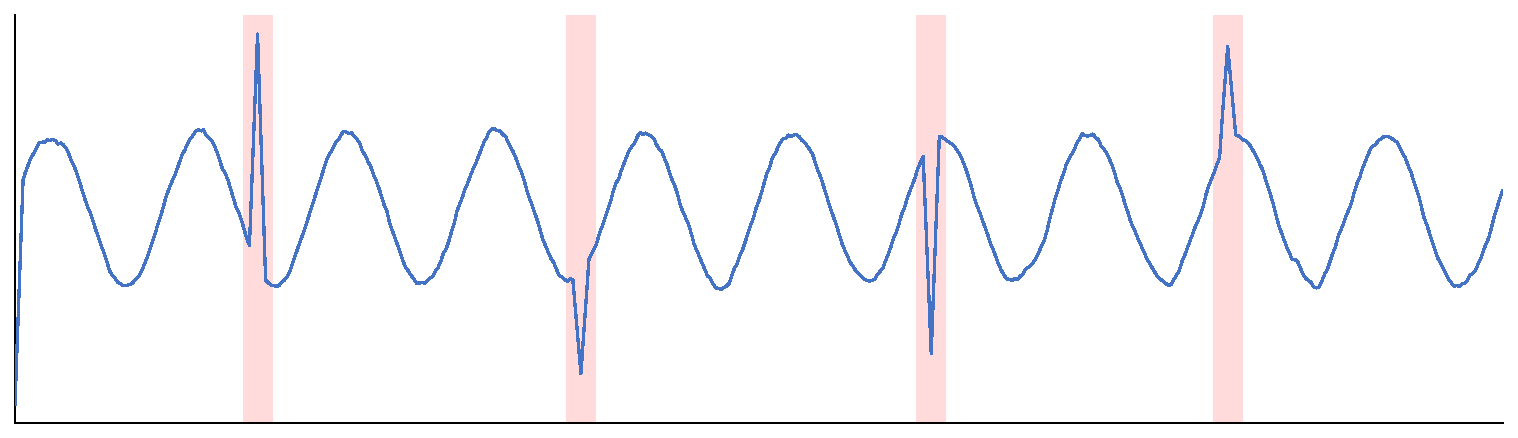
\includegraphics[width=0.92\textwidth]{Img/anomaly_type_a_point.pdf}
    \bicaption{\enspace 点异常示意图}{\enspace Illustration of Point Anomaly}
    \label{fig:anomaly_point}
\end{figure}

\textbf{第二类是片段异常（Subsequence Anomaly）}，也称为模式异常，指时间序列中一段连续数据点的行为显著偏离正常模式。与点异常不同，片段异常中的单个数据点可能并不构成异常，但整个子序列的模式与正常行为存在显著差异。根据异常模式的不同，片段异常可以细分为三种子类型：波形异常表现为振荡频率或幅度的突然改变，例如原本平稳的指标突然出现剧烈的高频震荡；季节性异常表现为周期性规律被打破，原有的周期结构在异常段内消失或发生显著变化；趋势异常则表现为序列的整体水平发生突变式的偏移，且偏移后的新水平在后续时间内持续保持。在分布式系统中，这类异常通常反映了较为持续的系统状态变化，如资源泄漏、配置错误或负载模式的异常转变。如图\ref{fig:anomaly_subsequence}所示，三个子图从上到下分别展示了波形异常、季节性异常和趋势异常的典型表现。

\begin{figure}[H]
    \centering
    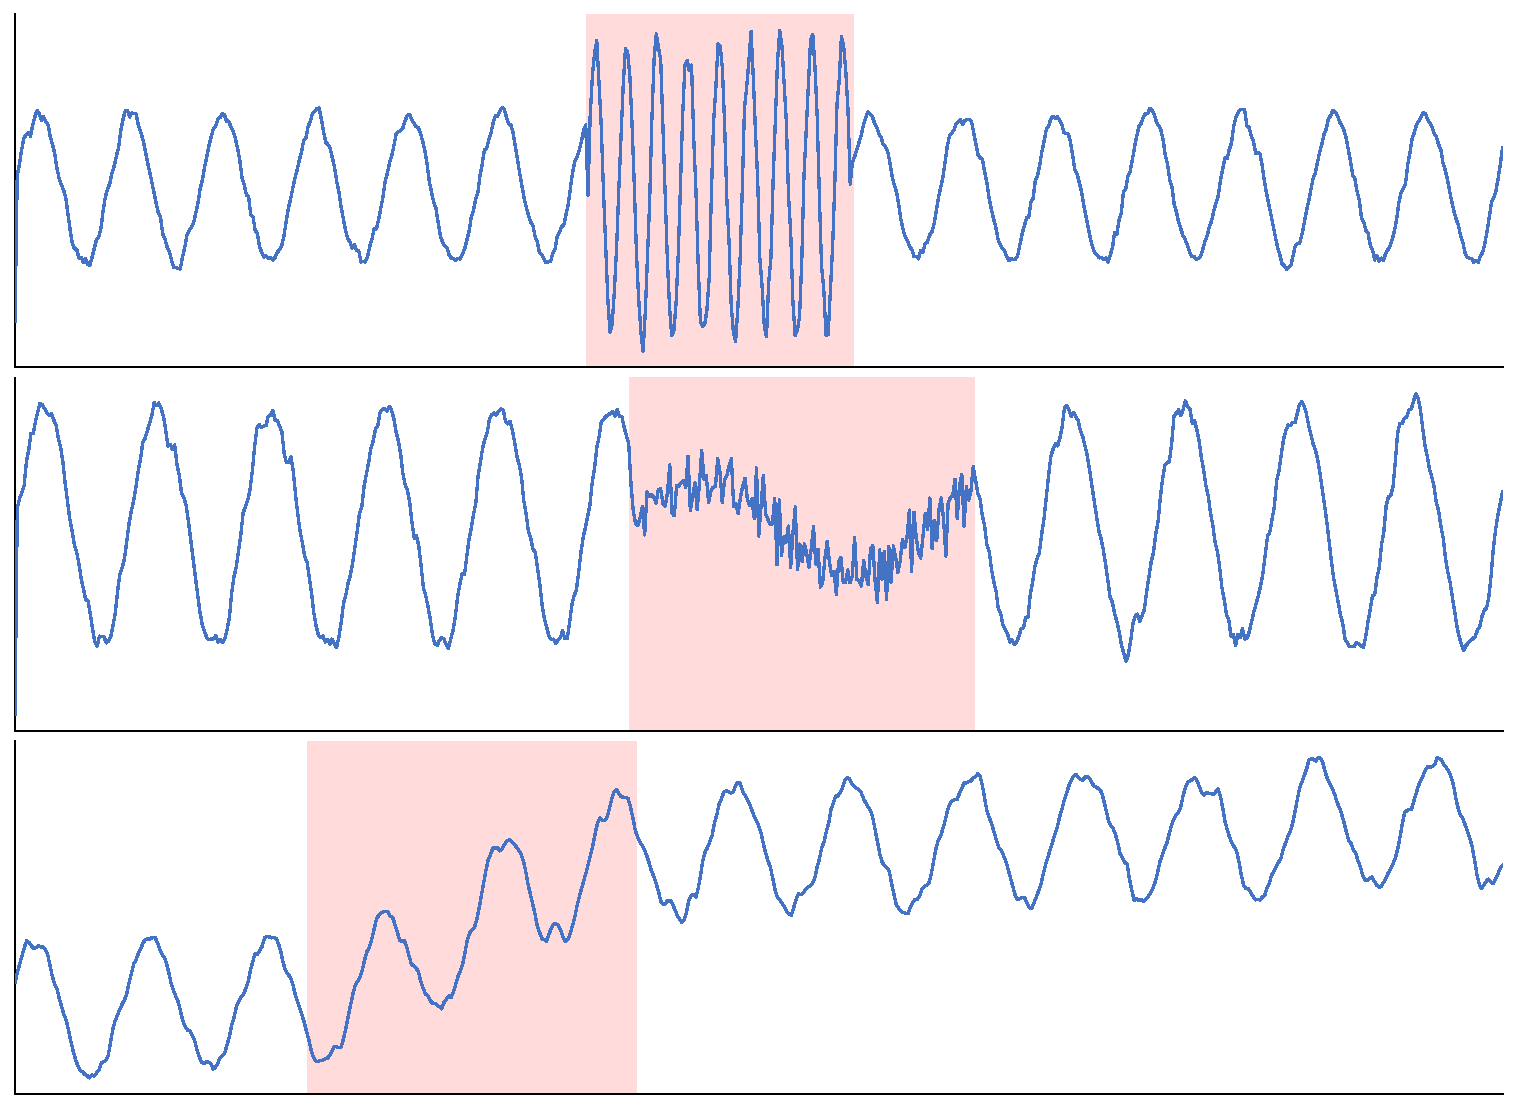
\includegraphics[width=0.85\textwidth]{Img/anomaly_type_b_subsequence.pdf}
    \bicaption{\enspace 片段异常示意图}{\enspace Illustration of Subsequence Anomaly}
    \label{fig:anomaly_subsequence}
\end{figure}

\textbf{第三类是变量间关联异常（Inter-variable Correlation Anomaly）}，这是多变量时间序列特有的异常类型，指变量间的关联关系随时间发生异常变化。在这类异常中，单个变量的数值可能均处于正常范围内，既不表现为点异常也不表现为片段异常，但变量之间原本稳定的关联模式（如正相关性、因果依赖）发生了显著偏离。例如，在正常运行状态下CPU使用率与网络吞吐量保持同步变化，而在异常状态下二者的关联关系可能反转或解耦。检测此类异常的核心难点在于需要同时建模时间维度上的演化规律和变量维度上的相互依赖关系，单纯基于单变量分析的方法难以发现这类隐蔽的异常。如图\ref{fig:anomaly_correlation}所示，两条曲线在正常区域保持同步波动，而在红色阴影区域内关联关系发生明显反转。

\begin{figure}[H]
    \centering
    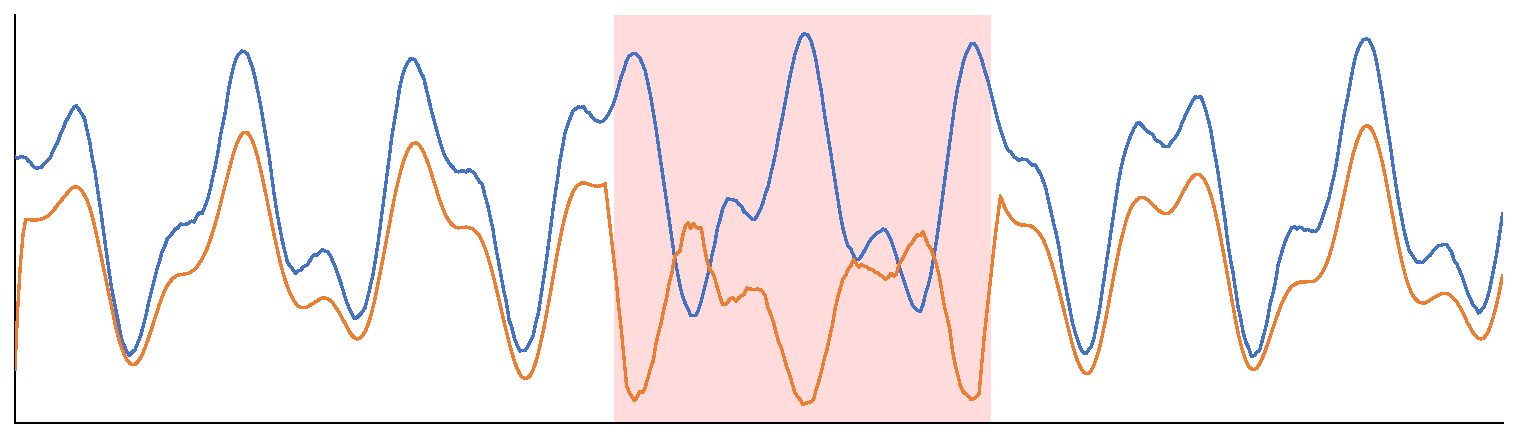
\includegraphics[width=0.92\textwidth]{Img/anomaly_type_c_correlation.pdf}
    \bicaption{\enspace 变量间关联异常示意图}{\enspace Illustration of Inter-variable Correlation Anomaly}
    \label{fig:anomaly_correlation}
\end{figure}

在分布式集群场景中，本文重点关注的是\textbf{节点级异常（Node-level Anomaly）}，即在多节点环境下，个别节点的监控曲线偏离集群整体行为模式的情形。在负载均衡机制的作用下，分布式集群中各节点承担的计算负载相近，其监控指标曲线通常表现出高度的形态相似性。当某个节点出现硬件退化、软件缺陷或配置偏差等问题时，其监控曲线会逐渐偏离正常节点群的行为模式，呈现出与群体不一致的演变趋势。这类异常的识别需要同时考虑时间维度的变化规律和节点维度的群体一致性，其本质是利用多节点之间的行为相似性作为正常基准，通过对比分析识别离群的异常节点。如图\ref{fig:anomaly_node}所示，多条蓝色曲线表示正常节点群的行为模式，红色曲线为异常节点，其在红色阴影区域内逐渐偏离正常节点群。

\begin{figure}[H]
    \centering
    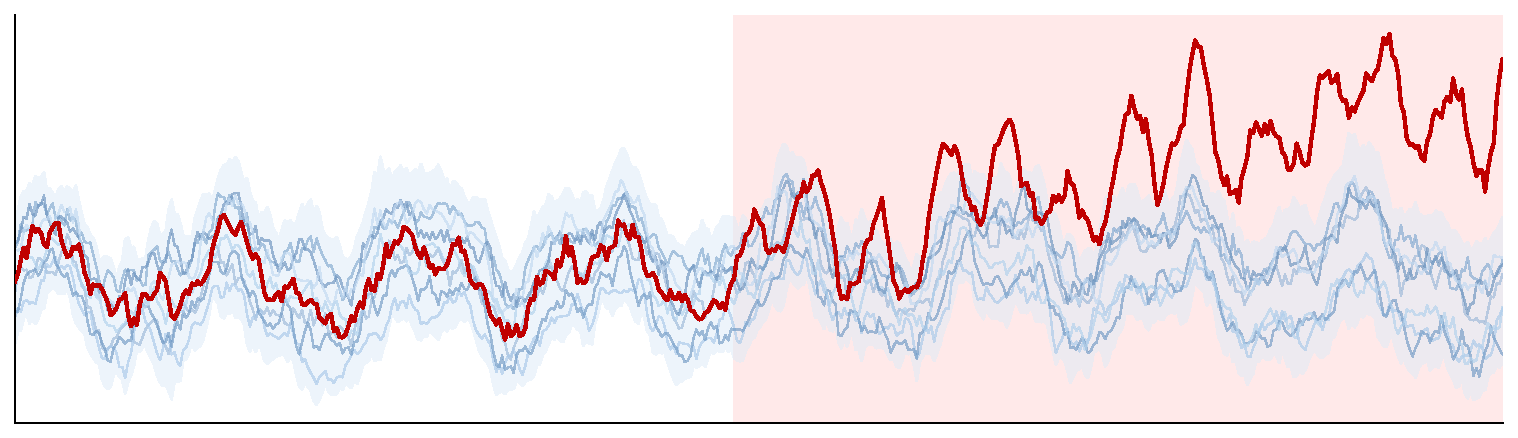
\includegraphics[width=0.92\textwidth]{Img/anomaly_type_d_node.pdf}
    \bicaption{\enspace 节点级异常示意图}{\enspace Illustration of Node-level Anomaly}
    \label{fig:anomaly_node}
\end{figure}

\section{时序异常检测算法}

时间序列异常检测方法可以从多个维度进行分类，主要包括学习范式、技术原理和数据维度。从学习范式角度，监督模式的选择取决于是否有标注数据：无监督方法（如孤立森林\cite{liu2008isolation}）无需任何标注数据，适用于新系统上线初期；半监督方法（如OCSVM、自编码器）仅需正常样本标注，在工业场景中最为常用；有监督方法则需要正常与异常样本均有标注，适用于已知特定异常模式的场景。

\subsection{单变量时序异常检测}

单变量时序异常检测旨在识别单条时间序列中的异常点或异常片段，其方法体系经历了从传统统计方法到经典机器学习方法再到深度学习方法的演进过程\cite{chandola2009anomaly,braei2020anomaly,blazquez2021review,chen2025tsadsurvey}。早期方法建立在概率分布假设和时序模型之上，随着数据规模和模式复杂度的增长，学习型方法逐渐成为主流。

传统统计方法在数据量适中、模式相对稳定时具有良好的理论基础和可解释性。基于分布假设的检验方法中，3-sigma准则假设数据服从正态分布，将落在$(\mu-3\sigma, \mu+3\sigma)$区间之外的点视为异常；Grubbs检验和ESD（Extreme Studentized Deviate test）则是专门为单变量数据设计的异常值统计检验方法\cite{chen2025tsadsurvey}。基于时序模型的预测方法以ARIMA（自回归综合移动平均）模型\cite{box1970arima}为代表，该方法通过差分将非平稳序列转化为平稳序列，再结合自回归（AR）和移动平均（MA）成分进行建模，将预测值与实际观测值的偏差超过设定阈值的点判定为异常。此外，分解方法如STL（Seasonal-Trend decomposition using Loess）\cite{cleveland1990stl}将时间序列分解为季节性、趋势性和残差三个部分，异常通常表现为残差分量中的极端值。这类传统方法原理简单、计算效率高、可解释性强，但其依赖于时序数据服从特定统计分布的假设，在面对复杂非线性模式时效果有限。

经典机器学习方法通过设计或选择特征度量，以无监督方式识别偏离正常模式的样本，不依赖于严格的分布假设。基于距离的方法如KNN（K近邻）通过计算数据点与其K个最近邻居的距离来识别异常。Breunig等人\cite{breunig2000lof}提出的LOF（局部离群因子）算法从局部密度角度出发，计算每个点相对于邻居的稀疏程度，值远大于1通常表示异常，该方法善于处理局部密度变化大的场景。Liu等人\cite{liu2008isolation}提出的孤立森林（Isolation Forest）因其高效性在工业界应用广泛，其核心思想是异常点``少且不同''，更容易在随机分割构成的树结构中被快速孤立出来，算法通过构建多棵隔离树并基于样本的平均路径长度计算异常分数。Sch{\"o}lkopf等人\cite{scholkopf2001ocsvm}提出的单类支持向量机（One-Class SVM）通过在特征空间中找到一个超平面来将正常数据与原点分离，偏离该边界的样本被判定为异常。此外，基于聚类的方法（如DBSCAN\cite{ester1996dbscan}、高斯混合模型等）将数据点分组，远离聚类中心或属于极小簇的点被视为异常。在保形预测框架方面，Ishimtsev等人\cite{ishimtsev2017conformal}提出了基于保形预测的k-NN异常检测器，通过保形理论为异常判断提供统计显著性保证，并支持在线增量处理，适用于流式数据的实时异常检测场景。Jin等人\cite{jin2019ocsvm}提出了基于一类支持向量机的时间序列变点检测校准方法，在标注样本稀缺的场景下展现了良好的检测效果。这些经典方法的共同优势在于无需大量标注数据且计算效率相对较高，但通常难以捕捉时间序列中复杂的非线性关系和长期时序依赖\cite{schmidl2022anomaly}。

近年来，深度学习方法凭借其强大的表征学习能力，在单变量时序异常检测领域取得了显著进展\cite{choi2021deepreview,pang2021deepsurvey,chalapathy2019deeplearning}。Hochreiter等人\cite{hochreiter1997lstm}提出的LSTM（长短期记忆网络）通过门控机制有效缓解了传统RNN的梯度消失问题，能够捕捉序列中的长期依赖关系；Chung等人\cite{chung2014gru}提出的GRU（门控循环单元）则通过简化门控结构在保持相近性能的同时降低了计算开销，两者均是时序建模中广泛使用的循环神经网络架构。Malhotra等人\cite{malhotra2015lstm}将LSTM应用于时序异常检测，使用历史正常数据训练模型进行多步预测，将显著的预测误差作为异常判据。自编码器（AutoEncoder）类方法通过编码器将输入压缩为低维潜在表示，再由解码器进行重构，当异常数据输入时会产生较大的重构误差，从而被识别。Zong等人\cite{zong2018dagmm}提出的DAGMM（深度自编码高斯混合模型）将自编码器的压缩表示与重构误差特征联合输入高斯混合模型进行端到端训练，有效避免了两阶段方法中特征提取与密度估计脱节的问题。Kingma等人\cite{kingma2014vae}提出的变分自编码器（VAE）进一步引入了对数据潜在分布的概率建模，Xu等人\cite{xu2018donut}在此基础上提出的Donut模型将VAE应用于周期性KPI的无监督异常检测，取得了良好效果。此外，基于GAN（生成对抗网络）的方法也被引入单变量时序异常检测，如BeatGAN\cite{zhou2019beatgan}通过对抗训练学习正常时序模式的生成模型，TadGAN\cite{geiger2020tadgan}结合了重构误差和评论者分数进行异常评分。Zhang等人\cite{zhang2024tfmae}提出的TFMAE（时频掩码自编码器）是应对训练数据含异常导致模型学习偏差这一挑战的创新方法，其核心是采用基于窗口的时间掩码和基于幅值的频率掩码两种策略，有选择地预消除输入中的潜在异常，通过最小化时间掩码表示与频率掩码表示之间的对比差异实现异常检测，对分布偏移更具鲁棒性。Wu等人\cite{wu2023timesnet}提出的TimesNet将一维时间序列变换为二维张量以捕捉周期内和周期间的二维变化模式，通过自适应发现多个周期并利用二维卷积提取复杂的时序特征，在包括异常检测在内的多项时间序列分析任务中表现优异。在实际部署方面，Yu等人\cite{yu2023autokad}提出的AutoKAD针对KPI异常检测中标签缺失导致的模型选择困难问题，设计了基于局部离群因子的无标签通用目标函数，实现了无需人工标注即可自动选择最优检测模型的能力。在模型架构方面，Zhou等人\cite{zhou2025kanad}提出的KAN-AD将Kolmogorov-Arnold网络引入时序异常检测，以截断傅里叶展开替代传统B样条基函数，结合轻量化学习机制强调全局模式，在多个基准数据集上取得了优异表现。深度学习方法的主要优势在于能自动捕获非线性与复杂依赖，但其局限性包括对数据量和计算资源需求高、超参数调优复杂以及模型决策可解释性不足\cite{chen2025tsadsurvey}。

\subsection{多元时序异常检测}

多元时序异常检测（Multivariate Time Series Anomaly Detection, MTSAD）旨在识别多个相关变量构成的时序数据中的异常模式。相较于单变量时间序列，多变量数据不仅包含每个变量自身随时间变化的模式，还蕴含了复杂的变量间关联关系，这既是其检测能力提升的潜力所在，也构成了核心挑战\cite{chen2025tsadsurvey}。当前多元时序异常检测方法主要可从重构、预测、图结构建模、因果分析和生成对抗等技术路线展开。

基于重构的方法是多元时序异常检测中最具代表性的范式之一。其核心思想是在正常数据上训练模型学习数据的低维表示，当异常数据输入时，由于其模式未被充分学习，会产生较大的重构误差。Su等人\cite{su2019omni}提出的OmniAnomaly采用随机变分自编码器和平面归一化流来学习多元时间序列的正常模式分布，通过重构概率识别异常，能够捕捉时间依赖性并建模正常数据的复杂分布。Audibert等人\cite{audibert2020usad}提出的USAD通过引入对抗性训练来增强自编码器的鲁棒性，从而提升重构误差对异常的敏感性。Malhotra等人\cite{malhotra2016lstmencoder}则提出了基于LSTM的编码器-解码器框架，利用LSTM的序列建模能力对多传感器数据进行重构，在多个工业数据集上展现了良好的异常检测性能。Chen等人\cite{chen2018autoencoder}将自编码器应用于网络流量异常检测，通过学习正常流量的低维表示并利用重构误差识别异常网络行为，验证了自编码器在网络安全领域的有效性。Park等人\cite{park2018lstmvae}提出了基于LSTM变分自编码器的多模态异常检测器，结合LSTM的时序建模能力和VAE的生成建模能力，通过联合建模多种传感器信号的时间依赖关系和概率分布实现异常检测。

基于预测的方法通过学习时间序列的时序演化规律，预测未来时刻的数值，将预测误差作为异常评分的依据。Tuli等人\cite{tuli2022tranad}提出的TranAD是一种基于深度Transformer的异常检测与诊断模型，它采用两阶段对抗训练机制：第一阶段生成输入窗口的近似重构，其重建损失作为第二阶段的关注分数；第二阶段利用此分数重新运行推理以放大重建误差，这种自调节机制有助于捕获鲁棒的多模态特征。Xu等人\cite{xu2022anomaly}提出的Anomaly Transformer通过关联差异性机制捕捉异常的时序特征，利用Transformer架构的强大自注意力机制捕捉时间序列长期依赖关系。Chen等人\cite{chen2023dcdetector}提出的DCdetector采用双重注意力对比表示学习，通过构建频域和时域的双通道注意力机制，增强了对细粒度异常模式的捕捉能力。Zhao等人\cite{zhao2020mtadgat}提出的MTAD-GAT结合了图注意力网络\cite{velickovic2018gat}和时间卷积网络，同时建模变量关联和时间依赖，是较早将图注意力引入多元时序异常检测的工作之一。

图神经网络（GNN）\cite{kipf2017gcn,wu2021gnnsurvey}天然适合对多变量时间序列中变量间的复杂关系进行显式建模。通过将变量视为图中的节点、关系视为边，GNN可以学习节点和边的表示，以识别异常节点或子图。Deng等人\cite{deng2021graph}提出的GDN通过学习传感器之间的图结构来检测异常，利用图神经网络传播信息并预测未来值，能够捕捉变量之间的复杂依赖关系。Dai等人\cite{dai2022graph}提出将图结构与归一化流相结合，通过图增强的归一化流模型对多变量时间序列的联合分布进行建模，为异常检测提供了概率论视角的解决方案。Zhang等人\cite{zhang2024gstpro}提出的GST-Pro针对现实中常存在缺失值的非规则采样多变量时间序列数据，基于神经控制微分方程对图时空过程进行建模，能够从空间和时间两个视角有效处理含缺失值的数据，并采用基于分布的异常评分机制。Liu等人\cite{liu2025mgcl}提出的MGCL专注于捕捉变量间的高阶交互关系，结合多尺度时序建模和自适应超图结构，以有效学习复杂的变量间和时序依赖关系。

从因果视角审视异常检测问题，将异常视为偏离了数据生成常规因果机制的实例，为提升检测的鲁棒性和可解释性提供了新思路。这类方法的核心创新在于将因果结构学习融入检测框架，利用因果系统的模块化特性，将复杂的多变量异常检测问题分解为一系列更简单的低维子问题，从而直接定位异常根源。Chen等人\cite{chen2025carots}提出的CAROTS创新性地将因果关系概念融入对比学习框架，设计了两种数据增强器：一种保留原始数据中的因果结构以生成代表正常波动的正样本，另一种则有意扰动因果关系以生成模拟异常行为的负样本，通过基于因果关系的对比学习训练编码器在潜在空间中有效区分正常与异常样本。Chen等人\cite{chen2025cgad}提出的CGAD利用转移熵构建变量间的因果图结构，并结合加权图卷积网络和因果卷积来同时捕捉因果与时间模式。

基于生成对抗网络（GAN）\cite{goodfellow2014gan}的方法利用生成器和判别器的对抗训练来学习正常数据分布。Li等人\cite{li2019madgan}提出的MAD-GAN将LSTM与GAN相结合，通过判别器得分和重构误差共同识别异常，是较早将GAN应用于多元时序异常检测的代表性工作。Ren等人\cite{ren2019srnn}在微软提出了面向大规模服务的时序异常检测方案，将谱残差方法与深度神经网络相结合，在实际生产环境中取得了良好效果。此外，Ca{\~n}izo等人\cite{canizo2019multihead}提出了多头CNN-RNN架构，通过为每个变量设置独立的卷积头提取局部特征，再经由共享的循环网络融合时序信息，在工业多时间序列异常检测中展现了良好的可扩展性。

近年来，将频域分析与时域分析相结合成为提升检测能力的重要方向。Wang等人\cite{wang2024fcvae}提出了频率增强条件变分自编码器（FCVAE），从频域视角重新审视VAE在无监督时序异常检测中的应用，通过引入频域增强机制有效捕捉不同频率成分中的异常特征。Zhang等人\cite{zhang2022tfad}提出的TFAD架构将时频分析与时间序列分解相结合，同时进行时域分解和频域分析，通过融合机制整合多视角的检测结果，在捕捉趋势性异常和周期性异常方面展现了优越的性能。

在面向运维场景的应用方面，He等人\cite{he2016loganalysis}从系统运维角度出发，提出了一种基于日志分析的异常检测方法，通过解析和结构化系统日志数据并利用机器学习模型识别日志中的异常模式，为分布式系统的故障诊断提供了有效手段。Ma等人\cite{ma2021jumpstarter}针对在线服务系统中频繁变更导致异常检测算法需要快速初始化的问题，提出了JumpStarter算法，结合形状聚类策略和抗异常值采样显著缩短了冷启动时间，有效应对了概念漂移场景下的检测挑战。

上述方法虽然在多元时序异常检测方面取得了显著进展，但主要关注时间维度和指标维度，未能充分利用分布式集群中多节点之间的行为相似性。本文的研究正是旨在弥补这一不足，将节点维度纳入异常检测的分析框架。

\section{分布式集群监控数据与异常检测}

\subsection{分布式集群概述}

分布式集群是融合了分布式系统与集群系统优势的计算架构，通过将任务分配到多个互相协作的服务器节点上，实现大规模数据的并行存储与处理。典型的分布式集群架构包括大数据领域的Hadoop集群和容器编排领域的Kubernetes集群等。作为支撑现代云计算与大数据处理的核心基础设施，分布式集群广泛应用于数据仓库、实时计算、机器学习训练等场景。此类集群的稳定运行直接关系到上层业务的连续性，因此对集群的监控和异常检测具有重要的实际意义。

以Hadoop分布式集群为例，其采用典型的主从（Master/Slave）架构，如图\ref{fig:hadoop_cluster}所示。在存储层，Hadoop分布式文件系统（HDFS）由一个NameNode主节点和多个DataNode工作节点组成。NameNode负责维护文件系统的元数据，如文件目录的布局和数据块的分布情况；DataNode处理数据块的物理存储，并通过多副本复制机制保证数据的可靠性。Secondary NameNode定期对NameNode的元数据进行检查点备份，以防止单点故障导致的数据丢失。在资源管理层，YARN（Yet Another Resource Negotiator）由ResourceManager和多个NodeManager组成。ResourceManager负责整个集群的资源调度和管理，NodeManager运行在各个计算节点上，负责管理节点的资源并执行容器化的计算任务。当用户通过客户端提交计算任务时，ResourceManager根据资源需求和调度策略将MapTask或ReduceTask分配到合适的节点上执行。为保证系统的可扩展性和容错性，Hadoop集群通常采用负载均衡机制，使得计算任务能够均匀分布到各个节点上。

\begin{figure}[H]
    \centering
    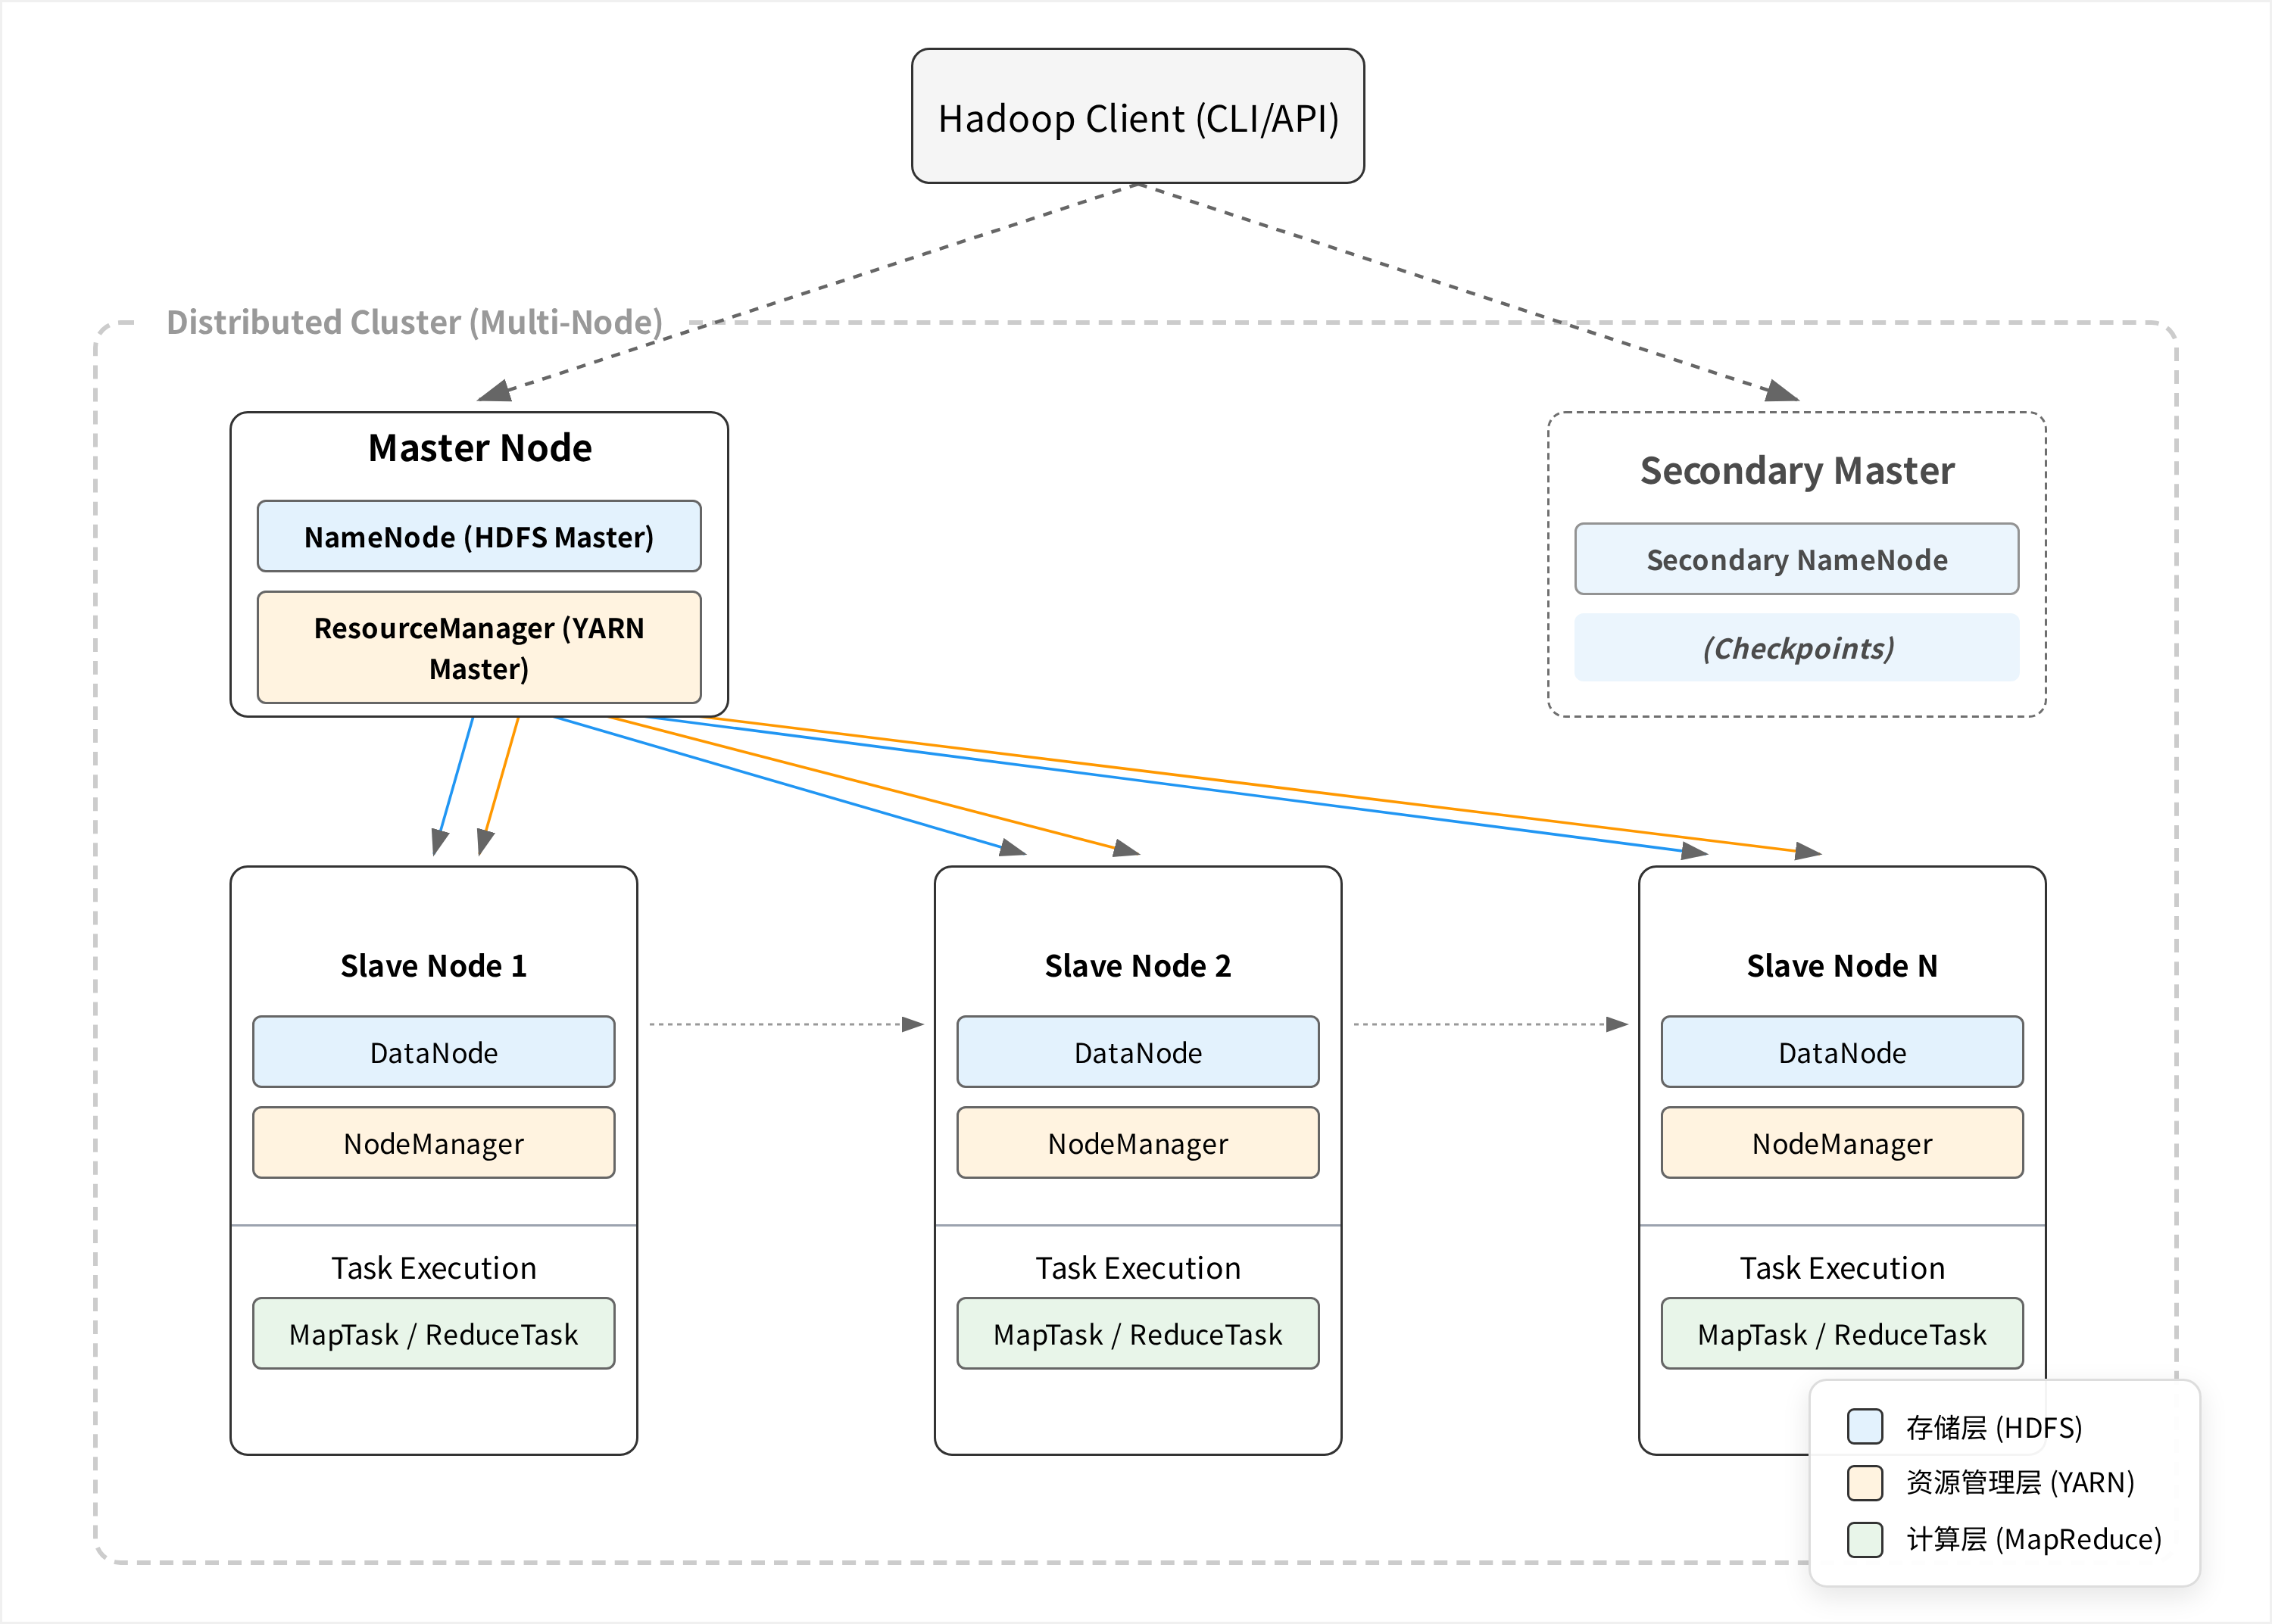
\includegraphics[width=0.88\textwidth]{Img/hadoop_html_render.png}
    \bicaption{\enspace Hadoop分布式集群架构示意图}{\enspace Architecture of Hadoop Distributed Cluster}
    \label{fig:hadoop_cluster}
\end{figure}

Hadoop集群的上述架构特征体现了分布式集群的核心设计理念：通过将存储与计算分布到多个节点上实现横向扩展能力，同时依靠副本机制和主从协调保障系统的可靠性。这些特征也决定了集群监控数据所呈现的独特模式，为后续异常检测方法的设计提供了重要背景。

\subsection{集群监控数据特点}

分布式集群在运行过程中会产生海量的多维度监控时序数据，这些数据具有若干显著特点。

多维度性是集群监控数据最突出的特点。集群监控涵盖多个层次和维度，包括系统级指标如CPU使用率和内存占用，应用级指标如请求响应时间和连接数，以及集群级指标如任务队列长度和资源使用率等，这些指标从不同角度反映系统的健康状态。

高频采样性则体现在数据的时间粒度上。为及时发现异常，监控系统通常以较高频率采集数据，常见的采样间隔为数秒到数分钟，由此产生的数据量巨大，对存储和处理提出了较高要求。

在空间维度上，集群数据具有显著的多节点相关性。由于负载均衡机制的作用，各节点在正常运行时承担的负载相近，其监控指标曲线往往表现出高度的形态相似性，这种相似性为基于群体一致性的异常检测提供了天然的基础。

另一方面，集群数据的动态波动性也不容忽视。与用户负载相关的指标具有正常模式难以统一定义的特点，其数值会随系统整体负载发生无规律波动，这种动态性增加了异常检测的难度，使得基于固定阈值或历史模式学习的方法容易产生误报。

\subsection{分布式异常检测系统架构}

随着数据规模的爆炸式增长，分布式集群环境下的时间序列异常检测成为必然趋势。传统的单机异常检测方法在处理大规模、高维度、实时性要求严格的场景时面临严重挑战，包括内存限制、计算瓶颈和可扩展性问题。分布式集群架构通过将计算任务和数据分布到多个节点上，实现了大规模时间序列异常检测的高效处理。

分布式多变量时间序列异常检测系统的架构设计主要遵循三种核心范式：

基于Spark的批处理系统架构采用弹性分布式数据集（RDD）作为核心数据抽象，通过内存计算优化大规模时间序列数据的离线分析。Spark框架的优势在于其强大的内存计算能力和容错机制，通过DAG调度器优化计算流程，支持迭代算法的高效执行\cite{fan2015spark}。

基于流处理的系统架构（如Apache Flink）专为实时时间序列异常检测设计，采用数据流作为核心抽象，支持有状态计算和事件时间处理。与基于批处理的Spark相比，流处理系统在低延迟流处理方面具有优势，能够满足对实时性要求极高的应用场景。

专门设计的分布式系统则针对特定算法或问题进行深度优化。例如，DADS（分布式异常检测系统）\cite{boniol2022dads}基于actor编程模型，将原始Series2Graph算法重构为反应式协议，通过异步消息传递和分布式计算实现了对单变量时间序列中序列异常的检测。

在数据分区策略方面，时间序列数据分区主要分为时间维度分区和变量维度分区两种模式。时间维度分区将长序列切分为等长的子序列片段，分配给不同计算节点处理。多变量数据的分区策略更为复杂，需要考虑变量间的相关性，基于变量聚类的分区策略有助于在并行计算时保持变量间的语义关联。

\subsection{异常检测方法在集群数据中的应用与挑战}

将现有时间序列异常检测方法应用于分布式集群监控数据时，面临来自数据特性、算法适配和应用需求等多个层面的挑战\cite{chen2025tsadsurvey}。本节从与本文研究密切相关的四个方面进行分析。

第一，正常基线缺失与概念漂移。传统异常检测方法通常假设存在可明确刻画的正常模式基线，然而分布式集群中与用户负载相关的监控指标（如CPU使用率、网络流量）其正常范围随集群整体负载动态变化，难以预先定义固定的正常区间。更重要的是，集群的运行模式会随业务迭代、版本升级、扩缩容等运维操作持续演变，即数据的生成分布随时间发生漂移\cite{chen2025tsadsurvey}。基于历史数据训练的检测模型容易将负载波动或正常的模式演变误判为异常，导致大量误报；同时，采样抖动和网络延迟引入的噪声进一步模糊了正常行为与异常行为之间的边界。这一挑战的本质在于：缺乏一种不依赖于绝对正常基线定义、且能适应数据分布动态变化的检测范式。

第二，节点维度信息利用不足。如2.2节所述，现有多元时序异常检测方法主要从时间维度和指标维度对数据进行建模，而未能有效利用分布式集群中多节点之间的行为相似性。在负载均衡机制的作用下，集群中各节点承担的计算负载相近，其同类监控指标曲线通常表现出高度的形态一致性。这种节点间的行为相似性蕴含了丰富的正常模式先验知识，为构建``群体行为基准''提供了天然的参照系，但目前尚缺乏系统化的方法来挖掘和利用这一维度的信息。

第三，标签稀缺与阈值自适应。在集群运维实践中，异常事件本身发生频率低且标注成本高昂，可用于模型训练和评估的标注数据极为稀缺\cite{chen2025tsadsurvey}。这一现状限制了有监督方法的适用性，要求检测算法具备在无标注或弱标注条件下有效工作的能力。此外，不同集群、不同指标、不同时段下的最优检测阈值差异显著，静态阈值难以适应动态变化的运行环境，亟需自适应的阈值确定机制。

第四，大规模数据的实时处理需求。分布式集群持续产生海量高频采样的监控数据，单机处理能力已无法满足大规模时序数据的实时分析需求\cite{boniol2022dads}。这要求检测系统在算法层面具备低计算复杂度，在架构层面支持分布式并行处理，同时满足故障及时发现的实时性约束。

针对上述挑战，本文的核心思路是利用分布式集群多节点曲线的行为相似性构建异常检测方法。在负载均衡机制下，正常节点的监控曲线应保持较高的形态相似性，而异常节点的曲线会显著偏离群体行为模式。基于这一观察，通过对比节点间的曲线差异识别离群的异常节点，能够绕过正常基线定义困难的问题；同时，设计自适应阈值机制应对标签稀缺与阈值选择的挑战，并基于分布式计算框架实现大规模数据的高效处理。

\section{本章小结}

本章系统介绍了时间序列异常检测的相关背景知识与理论基础。在异常概念层面，阐述了时间序列异常数据的基本特征，并对异常类型进行了系统分类，包括点异常、片段异常、变量间关联异常和节点级异常。在算法层面，回顾了单变量和多元时序异常检测的主流方法，涵盖从传统统计方法、经典机器学习方法到深度学习方法的发展脉络，重点介绍了基于重构、预测、图神经网络和因果分析的多元时序异常检测方法。在应用层面，介绍了分布式集群的基本概念、监控数据特点和分布式异常检测系统架构，并从正常基线缺失与概念漂移、节点维度信息利用不足、标签稀缺与阈值自适应、大规模数据实时处理等方面分析了现有方法在集群场景中面临的关键挑战，明确了本文的研究切入点。本章内容为后续章节的算法设计奠定了理论基础。
